% Document notes:
% For the figures showing the grids with current coming into the page, would like to create a space so the "x" isn't colliding with the tick marks
\documentclass [12pt, letterpaper, twoside]{article}
\usepackage[utf8]{inputenc}
\usepackage [left=1.0in, right=1.0in, top=1.0in, bottom=1.0in]{geometry}
% For updated time
\usepackage{datetime}
% For drawing pictures
\usepackage{tikz}
% For equations
\usepackage{amsmath}
% To make tables
\usepackage{tabu}
% For multiple rows in table slot
\usepackage{multirow}
% To add captions
\usepackage{caption}
% Forget what this is for
\usepackage{float}
% To make graphs
\usepackage{pgfplots}
% To make scatter plots
\usepackage{pgfplotstable}
%\usepackage[siunitx, RPvoltages]{circuitikzgit}
% To make tables side by side
\usepackage{subfig}
% To make inline fractions
\usepackage{xfrac}
% To make hyperlinks
\usepackage{hyperref}
% To make degree symbol
\usepackage{gensymb}

\usetikzlibrary{shapes.geometric}

% Drawing the magnet
\tikzset{
  outPage/.pic = {
    % The magnet dimensions
    \def\lmag{1.0}
    \def\wmag{0.25}
    % Placement of the first magnet (at (0,1.5))
    \coordinate (A) at (-\lmag/2,\wmag/2+1.5);
    \coordinate (B) at (0,-\wmag/2+1.5);
    % Coloring in the first magnet with poles
    \draw[fill,color=blue](A) rectangle ++(\lmag/2,-\wmag);
    \draw[fill,color=red](B) rectangle ++(\lmag/2,\wmag);
             },
  inPage/.pic = {
    % The magnet dimensions
    \def\lmag{1.0}
    \def\wmag{0.25}
    % Placement of the first magnet (at (0,1.5))
    \coordinate (A) at (-\lmag/2,\wmag/2+1.5);
    \coordinate (B) at (0,-\wmag/2+1.5);
    % Coloring in the first magnet with poles
    \draw[fill,color=red](A) rectangle ++(\lmag/2,-\wmag);
    \draw[fill,color=blue](B) rectangle ++(\lmag/2,\wmag);
            }
         }

\raggedbottom
\pgfplotsset{compat=1.16}
\begin{document}
\begin{titlepage}
\begin{center}
College of Science: Physics Department \\
\vspace{0.1cm}
Illinois Institute of Technology\\
\vspace{0.1cm}
General Physics II: Electromagnetism (PHYS 221-01)\\
\vspace*{\fill}
\begingroup
\Large
\textbf{Magnetic Fields and Forces}
\vspace{0.35cm}

\normalsize
Lab 8
\vspace{1.5cm}
\endgroup
\vspace*{\fill}
\end{center}

\vspace*{\fill}
\begin{flushright}
\footnotesize
Emily Pang \\
Date of experiment: 1 Apr 2020 \\
Due date: 8 Apr 2020 \\
Lab section L06 \\
TA: Will Limestall \\
Updated \usdate\today~(\currenttime)
\end{flushright}
\end{titlepage}
\subsection*{STATEMENT OF OBJECTIVE}
The objective of this lab was to observe the magnetic field as a result of a current-carrying wire, as well as measure the force exerted on a magnet from a current-carrying wire.

\subsection*{THEORY}
Current is defined as the rate of electric charge through a material. When this material is then placed in a magnetic field, a magnetic force is exerted on it. This force is represented as:
\begin{equation*}
  \begin{split}
    \vec{F} &= q\vec{v}\times{\vec{B}} \\
  \end{split}
\end{equation*}
where \(q\) represents the charge of the particle moving through the magnetic field, \(\vec{v}\) is the velocity of said particle, and \(\vec{B}\) is the magnetic field. Note that \(\vec{v}\) and \(\vec{B}\) are vectors being multiplied as a cross-product, so the force should also be a vector. To obtain the force acting on a wire and not just a particle, the force is multiplied by the number of charges in the wire:
\begin{equation*}
  \begin{split}
    \vec{F}_{\text{wire}} &= (nAL)(q\vec{v}\times{\vec{B}}) \\
  \end{split}
\end{equation*}
where \(nAL\) is the number of charges going through the entirety of the wire.

\noindent
However, examining a wire requires taking into consideration the culmination of the moving charges in the wire, using
\begin{equation}
  \begin{split}
    I &= nqvA \\
    qv &= \dfrac{I}{nA} \\ 
  \end{split}
\end{equation}
where \(n\) is the number of charges per unit volume, \(A\) is the cross-sectional area of the material, \(q\) is the charge of each particle, and \(v\) is the velocity of the charges through the material. Then \(qv\) is equal to the current divided by \(nA\). Combining the two equations gives:
\begin{equation}
  \begin{split}
    \vec{F}_{\text{wire}} &= (nAL)\left(\dfrac{I}{nA}\times{\vec{B}}\right) \\
    \vec{F}_{\text{wire}} &= I\vec{L}\times\vec{B} \\
  \end{split}
\end{equation}

\noindent
The magnitude of this force is given by:
\begin{equation*}
  \begin{split}
    |\vec{F}_{\text{wire}}| = ILB\sin(\theta) \\
  \end{split}
\end{equation*}
where \(\theta\) is the angle between \(\vec{L}\) and \(\vec{B}\). When \(\theta\) is equal to \(90\degree\), then the \(\sin(\theta)\) effectively disappears. In the second part of the lab, this is the case. Thus, if the results were to be graphed, \(|\vec{F}_{\text{wire}}|\) would represent the \(y\)-value, \(I\) would be the \(x\)-value, and \(LB\) would be the slope of the best-fit line. It could also be graphed where \(IB\) is the slope of the best-fit line if \(L\) and \(|\vec{F}_{\text{wire}}|\) are known. Then \(|\vec{F}_{\text{wire}}|\) would be the \(y\)-value and \(L\) would be the \(x\)-value.

\subsection*{EQUIPMENT}
  \noindent
  \begin{itemize}
    \itemsep0em
    \item{one wire}
    \item{one power supply}
    \item{one ammeter}
    \item{one stand to hold the wire}
    \item{one PASCO Capstone Sensor and associated software}
    \item{wires to connect power supply and stand}
    \item{horseshoe magnet}
  \end{itemize}

\subsection*{PROCEDURE}
The first part of the experiment involved drawing out the observed magnetic fields when placing a compass near the wire held in the stand while it carried current. The current was set to 5.0 Amps. Near the bottom of the stand was a platform depicting the following shown in Figure 1. The compass was then moved around while its position and reaction were recorded.

\noindent
The second part of the lab involved demonstrating the magnetic force varying the current and the length of the wires. For each of these parts, the magnetic force was calculated from the effect the current through the wires had on the mass of the horseshoe magnet.

\subsection*{DATA}
Figures ~\ref{fig:1} and ~\ref{fig:2} show the orientation of the north and south poles of the compass as it was placed in eight different orientations around the platform with the wire. Figure 1 shows the north poles facing clockwise, while Figure 2 shows the north poles facing counter-clockwise.

\noindent
The specifications for the horseshoe magnet are shown in Figure ~\ref{fig:3}. The mass of the magnet as the longest wire with a varying current is placed between its poles is shown in Table 1. Table ~\ref{fig:tab2} shows the different wires, their lengths, and their effect (by changing mass) on the magnet as a current of 5 Amps was put through the wires.

\begin{figure}
  \centering
  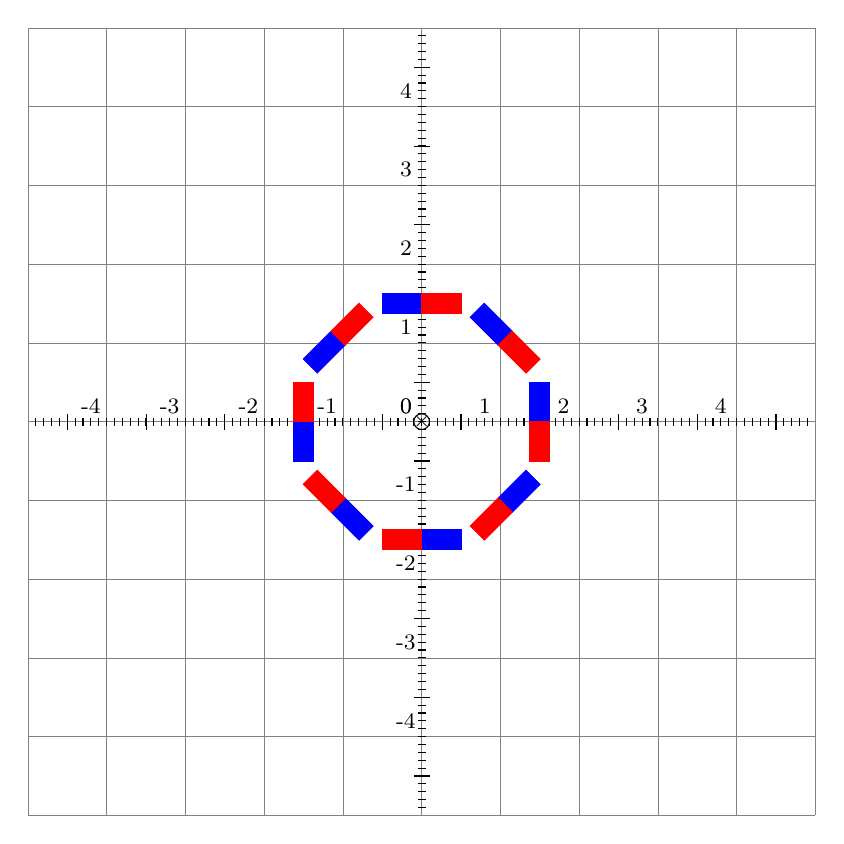
\begin{tikzpicture}
    \draw[step=1cm,gray,very thin] (-5,-5) grid (5,5);
    % Label numbers on x-line
    \foreach \xnumber in {-4,...,4}
    \node at (\xnumber - 0.20, 0.20) {\footnotesize{\xnumber}};
    % Label numbers on y-line
    \foreach \ynumber in {-4,...,4}
    \node at (- 0.20, \ynumber + 0.20) {\footnotesize{\ynumber}};
    % Medium tick marks on x-line 
    \foreach \xmediumtick in {-5,...,4}
    \draw (-0.1,\xmediumtick + 0.5) -- (0.1,\xmediumtick + 0.5);
    % Medium tick marks on y-line
    \foreach \ymediumtick in {-5,...,4}
    \draw (\ymediumtick + 0.5,0.10) -- (\ymediumtick + 0.5,-0.10);
    % Small tick marks on x-line
    \foreach \xsmalltick in {-49,...,49}
    \draw (-0.05,0.1*\xsmalltick) -- (0.05,0.1*\xsmalltick);
    % Small tick marks on y-line
    \foreach \ysmalltick in {-49,...,49}
    \draw (0.1*\ysmalltick,-0.05) -- (0.1*\ysmalltick,0.05);
    % Current in wire
    \draw (0,0) circle (0.1cm);
    % Show current going into the page
    \node at (0,0) {\scriptsize{\(\times\)}};
    % Draw magnets in circle around origin
    \foreach \rotatenum in {0,...,8}
    \path pic {outPage} pic[rotate=\rotatenum*45] {outPage};
    %\node[circle,draw,line width=0.1cm,minimum size=3.0cm] at (0,0) {};
  \end{tikzpicture}
  \caption{Mapped Magnetic Field (Part 1), Current In Page}
  \label{fig:1}
\end{figure}

\begin{figure}
  \centering
  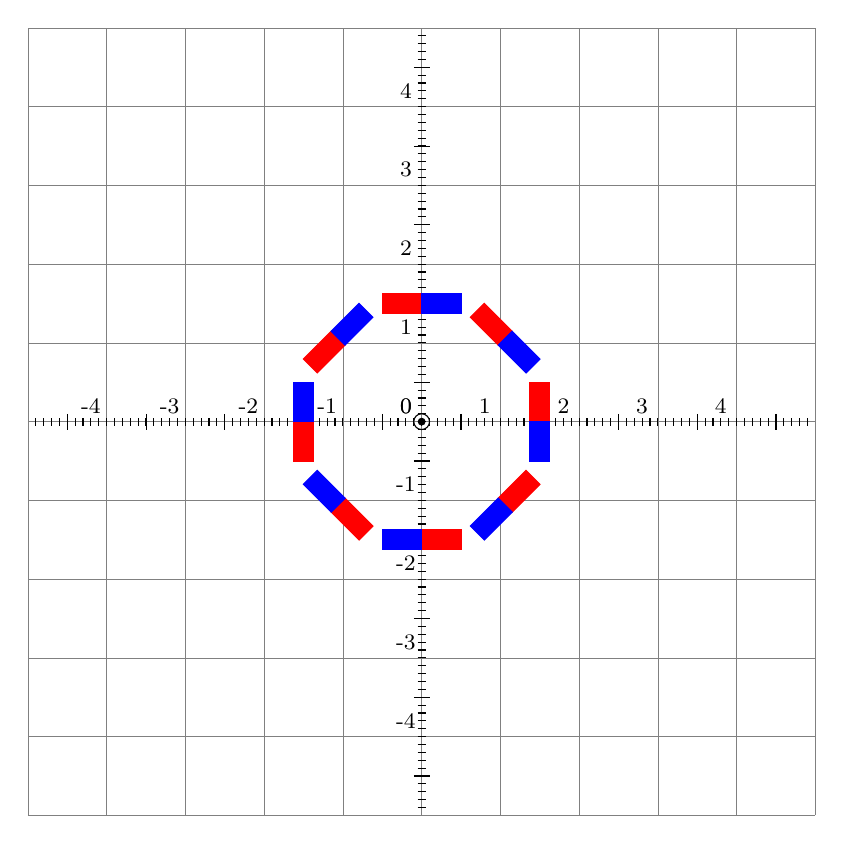
\begin{tikzpicture}
    \draw[step=1cm,gray,very thin] (-5,-5) grid (5,5);
    % Label numbers on x-line
    \foreach \xnumber in {-4,...,4}
    \node at (\xnumber - 0.20, 0.20) {\footnotesize{\xnumber}};
    % Label numbers on y-line
    \foreach \ynumber in {-4,...,4}
    \node at (- 0.20, \ynumber + 0.20) {\footnotesize{\ynumber}};
    % Medium tick marks on x-line 
    \foreach \xmediumtick in {-5,...,4}
    \draw (-0.1,\xmediumtick + 0.5) -- (0.1,\xmediumtick + 0.5);
    % Medium tick marks on y-line
    \foreach \ymediumtick in {-5,...,4}
    \draw (\ymediumtick + 0.5,0.10) -- (\ymediumtick + 0.5,-0.10);
    % Small tick marks on x-line
    \foreach \xsmalltick in {-49,...,49}
    \draw (-0.05,0.1*\xsmalltick) -- (0.05,0.1*\xsmalltick);
    % Small tick marks on y-line
    \foreach \ysmalltick in {-49,...,49}
    \draw (0.1*\ysmalltick,-0.05) -- (0.1*\ysmalltick,0.05);
    % Current in wire
    \draw (0,0) circle (0.1cm);
    % Show current going out of the page
    \fill[black] (0,0) circle (0.05cm);
    % Draw magnets all around
    \foreach \rotatenum in {0,...,8}
    \path pic {inPage} pic[rotate=\rotatenum*45] {inPage};
  \end{tikzpicture}
  \caption{Mapped Magnetic Field (Part 1), Current Out of Page}
  \label{fig:2}
\end{figure}

\begin{figure}
  \centering
  \subfloat[Strength of Magnet]{
    \begin{tabular}{| c | c |}
      \hline\hline
      Side & Magnetic Field Strength (T) \\
      \hline
      Red & 0.0224 \(\pm\) 0.0002 \\
      \hline
      Blue & -0.0223 \(\pm\) 0.0002 \\
      \hline\hline
    \end{tabular}
  }\qquad
  \subfloat[Mass of Magnet]{
    \begin{tabular}{| c | c |}
      \hline\hline
      Trials & Mass (kg) \\
      \hline
      1 & 0.16275 \\
      \hline
      2 & 0.16274 \\
      \hline
      3 & 0.16275 \\
      \hline
      Average & 0.16275 \\ % 6667 (LDR)
      \hline\hline
    \end{tabular}
  }
  \caption{Magnet Specifications}
  \label{fig:3}
\end{figure}

\begin{table}
  \centering
  \begin{tabular}{| c | c | c | c | c |}
    \hline\hline
    Current (A) & Mass (kg) & Average Mass (kg) & Net Mass (kg) & \(F_{\text{magnetic}}\) (N) \\
    \hline
    \multirow{3}{*}{0.50} & 0.16302 & & & \\
    & 0.16302 & 0.16302 & 0.000273333 & 0.002678663 \\
    & 0.16302 & & & \\
    \hline
    \multirow{3}{*}{1.00} & 0.16332 & & & \\
    & 0.16332 & 0.16332 & 0.000573333 & 0.005618663 \\
    & 0.16332 & & & \\
    \hline
    \multirow{3}{*}{1.50} & 0.16361 & & & \\
    & 0.16361 & 0.16361 & 0.000866667 & 0.008493337 \\
    & 0.16362 & & & \\
    \hline
    \multirow{3}{*}{2.00} & 0.16390 & & & \\
    & 0.16391 & 0.16390 & 0.001156667 & 0.011335337 \\
    & 0.16390 & & & \\
    \hline
    \multirow{3}{*}{2.50} & 0.16419 & & & \\
    & 0.16419 & 0.16419 & 0.001443333 & 0.014144663 \\
    & 0.16419 & & & \\
    \hline
    \multirow{3}{*}{3.00} & 0.16448 & & & \\
    & 0.16448 & 0.16448 & 0.001733333 & 0.016986663 \\
    & 0.16448 & & & \\
    \hline
    \multirow{3}{*}{3.50} & 0.16477 & & & \\
    & 0.16477 & 0.16477 & 0.002023333 & 0.019828663 \\
    & 0.16477 & & & \\
    \hline
    \multirow{3}{*}{4.00} & 0.16507 & & & \\
    & 0.16506 & 0.16506 & 0.002316667 & 0.022703337 \\
    & 0.16506 & & & \\
    \hline
    \multirow{3}{*}{4.50} & 0.16536 & & & \\
    & 0.16535 & 0.16535 & 0.002603333 & 0.025512663 \\
    & 0.16534 & & & \\
    \hline
    \multirow{3}{*}{5.00} & 0.16564 & & & \\
    & 0.16564 & 0.16564 & 0.00289 & 0.028322 \\
    & 0.16563 & & & \\
    \hline\hline
  \end{tabular}
  \caption{Mass of Magnet with Varying Currents Through Wire}
  \label{fig:tab1}
\end{table}

\begin{table}
  \centering
  \begin{tabular}{| c | c | c | c | c |}
    \hline\hline
    Current Loop & Length (m) & Mass (kg) & Net Mass (kg) & \(F_{\text{magnetic}}\) (N) \\
    \hline
    \multirow{3}{*}{SF 40} & & 0.16312 & & \\
    & 0.012 & 0.16312 & 0.000373333 & 0.003658667 \\
    & & 0.16312 & & \\
    \hline
    Average & & 0.16312 & & \\
    \hline
    \multirow{3}{*}{SF 37} & & 0.16348 & & \\
    & 0.022 & 0.16348 & 0.000733333 & 0.007186667 \\
    & & 0.16348 & & \\
    \hline
    Average & & 0.16348 & & \\
    \hline
    \multirow{3}{*}{SF 39} & & 0.16386 & & \\
    & 0.032 & 0.16386 & 0.001113333 & 0.010910667 \\
    & & 0.16386 & & \\
    \hline
    Average & & 0.16386 & & \\
    \hline
    \multirow{3}{*}{SF 38} & & 0.16425 & & \\
    & 0.042 & 0.16425 & 0.001503333 & 0.014732667 \\
    & & 0.16425 & & \\
    \hline
    Average & & 0.16425 & & \\
    \hline
    \multirow{3}{*}{SF 41} & & 0.16482 & & \\
    & 0.064 & 0.16482 & 0.002073333 & 0.020318667 \\
    & & 0.16482 & & \\
    \hline
    Average & & 0.16482 & & \\
    \hline
    \multirow{3}{*}{SF 42} & & 0.16561 & & \\
    & 0.084 & 0.16561 & 0.002863333 & 0.028060667 \\
    & & 0.16561 & & \\
    \hline
    Average & & 0.16561 & & \\
    \hline\hline
  \end{tabular}
  \caption{Wires, their lengths, and mass of magnet as result}
  \label{fig:tab2}
\end{table}

\subsection*{ANALYSIS OF DATA}
For the first part of the experiment, Figure 1 shows that the magnetic field is going clockwise, as demonstrated by the position of the north poles. Using the Right Hand Rule (RHR), if the current is pointing into the page, the magnetic field is going clockwise. 

\noindent
For Figure 2, the current was reversed and came out of the page. The direction of the north poles also reversed, showing the magnetic field as pointing counter-clockwise. By the same RHR, the magnetic field must be going counter-clockwise.

\noindent
For the second part of the experiment, the length of the wire was kept constant while the current running through it was varied, as shown in Table ~\ref{fig:tab1}. As the current increased, the mass of the magnet increased. Figure ~\ref{fig:4} shows an FBD of the horseshoe magnet. Notice that the magnetic and gravitational forces on the magnet are equal to the normal force, showing there is no acceleration when the mass was measured. The magnetic force can be found by two ways. First, by Figure 4, the normal force is equal to \(F_{\text{gravity}} + F_{\text{magnetic}}\), so \(F_{\text{magnetic}}\) can be found by subtracting \(F_{\text{gravity}}\). This process is demonstrated below:
\begin{equation*}
  \begin{split}
    F_{\text{normal}} &= F_{\text{gravity}} + F_{\text{magnetic}} \\
    F_{\text{magnetic}} &= F_{\text{normal}} - F_{\text{gravity}} \\
    F_{\text{magnetic}} &= (\text{new mass})(9.8 \sfrac{\text{m}}{\text{s}^{2}}) - (\text{mass})(9.8 \sfrac{\text{m}}{\text{s}^{2}}) \\
    F_{\text{magnetic}} &= (9.8\sfrac{\text{m}}{\text{s}^{2}})(\text{new mass} - \text{mass}) \\
  \end{split}
\end{equation*}
Table 1 demonstrates the above process to plot Figure ~\ref{fig:5} with a best-fit line of \(y = 0.00569x - 8.49\cdot{10}^{-2}\). As shown earlier in the theory section, the slope of the best-fit line should be approximately equal to \(LB\), the product of the length of the wire and the magnetic field. The strength of the magnetic field of the magnets can be found by solving for \(B\):
\begin{equation*}
  \begin{split}
    B &= \dfrac{\text{slope}}{L} \\
      &= \dfrac{0.00569\text{T}\cdot\text{m}}{0.084\text{m}} \\
      &= 0.067738095 \\
  \end{split}
\end{equation*}

\noindent
When the magnets are together (as between the poles of the horseshoe magnet), the magnetic field is doubled. Thus, the percentage difference was calculated as such:

\begin{equation*}
  \begin{split}
    \%\text{ Difference} &= \dfrac{0.0677 - (2)(0.02235)}{\tfrac{0.0677 + (2)(0.02235)}{2}}\cdot{100} \\
    \%\text{ Difference} &= 41.0\% \\ %791628 (LDR)
  \end{split}
\end{equation*}

\noindent
The strength of the magnetic field can be found again using the same process as before for the second half of the second part. \(IB\) represents the slope of the best-fit line when the length of the wire is varied as shown in Figure ~\ref{fig:6}. Thus:
\begin{equation*}
  \begin{split}
    B &= \dfrac{\text{slope}}{I} \\
      &= \dfrac{0.33094(\text{T}\cdot{A})}{5\text{A}} \\  
      &= 0.066188\text{ T} \\
  \end{split}
\end{equation*}

\noindent
The percentage difference for this result is:
\begin{equation*}
  \begin{split}
    \%\text{ Difference} &= \dfrac{0.0662 - (2)(0.02235)}{\tfrac{0.0662 + (2)(0.02235)}{2}}\cdot{100} \\
    \%\text{ Difference} &= 38.8\% \\ %5622249 (LDR)
  \end{split}
\end{equation*}

\begin{figure}
  \centering
  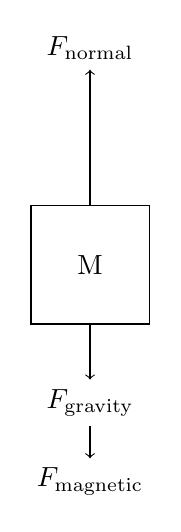
\begin{tikzpicture}
    \tikzstyle{magnet}=[rectangle,draw,minimum size=1.5cm]
    \node (magnet) at (0,0) [magnet] {M};
    \node (NForce) at (0,2.75) {\(F_{\text{normal}}\)};
    \node (GForce) at (0,-1.75) {\(F_{\text{gravity}}\)};
    \node (BForce) at (0,-2.75) {\(F_{\text{magnetic}}\)};
    \draw [->] (magnet) -- (NForce);
    \draw [->] (magnet) -- (GForce);
    \draw [->] (GForce) -- (BForce);
  \end{tikzpicture}
  \caption{Free Body Diagram of horseshoe magnet}
  \label{fig:4}
\end{figure}

\pgfplotstableread{
X Y
0.50 2.678663
1.00 5.618663
1.50 8.493337
2.00 11.335337
2.50 14.144663
3.00 16.986663
3.50 19.828663
4.00 22.703337
4.50 25.512663
5.00 28.322
}\currentForce

\begin {figure}                                                             
  \centering
  \begin{tikzpicture}
%    \draw[color=blue] plot (\x,7.585\e^{-\x/48.5});
    \begin{axis}[
      title = {Current Through Wire and Magnetic Force},
      xlabel = {Current (A)},
      ylabel = {\(F_{\text{magnetic}}\) (mN)},
      legend pos = north west,
      ]
      \addplot [only marks, mark = *] table {\currentForce};
      \addplot [thick, red] table[
        y={create col/linear regression={y=Y}}
      ]
      {\currentForce};
      \addlegendentry{Data}
      \addlegendentry{\((\pgfmathprintnumber{\pgfplotstableregressiona})x\pgfmathprintnumber[print sign]{\pgfplotstableregressionb}\)};
    \end{axis}
  \end{tikzpicture}
  \caption{}
  \label{fig:5}
\end{figure}

\pgfplotstableread{
X Y
0.012 3.658667
0.022 7.186667
0.032 10.910667
0.042 14.732667
0.064 20.318667
0.084 28.060667
}\forceLength

\begin{figure}                                                             
  \centering
  \begin{tikzpicture}
%    \draw[color=blue] plot (\x,7.585\e^{-\x/48.5});
    \begin{axis}[
      title = {Current Through Wire and Length of Wire},
      xlabel = {Length of Wire (m)},
      ylabel = {\(F_{\text{magnetic}}\) (mN)},
      legend pos = north west,
      ]
      \addplot [only marks, mark = *] table {\forceLength};
      \addplot [thick, red] table[
        y={create col/linear regression={y=Y}}
      ]
      {\forceLength};
      \addlegendentry{Data}
      \addlegendentry{\((\pgfmathprintnumber{\pgfplotstableregressiona})x\pgfmathprintnumber[print sign]{\pgfplotstableregressionb}\)};
    \end{axis}
  \end{tikzpicture}
  \caption{}
  \label{fig:6}
\end{figure}

\subsection*{DISCUSSION OF RESULTS}
For the first part of the experiment, the results obtained were expected. When the current switched directions, the direction the north pole of the compass also changed, and corresponded to the RHR.

For the second part of the experiment when varying the current, the results obtained numerically corresponded with what was expected (that the magnetic force increased as the current increased). However, the percentage difference was fairly high, at 41.0\%. This large difference could be due to general disposition of the experiment, as the values obtained were small and could easily be affected by other magnetic fields. 

\noindent
For the last part when varying the length of the wires between the magnet, the results again agreed with the expectation that with more wire, the overall charges flowing between the magnet would increase. While the value for the magnetic field was very similar to the magnetic field calculated previously, it still had a high percentage difference. Again, this high percentage difference could be due to outside magnetic fields. 

\noindent
Note that while the current loop contained segments 2-3, 3-4, and 4-5, only the loop from 3-4 actually contributed. For instance, referencing the RHR, the forces of the wires cancel out, as the currents are going in opposite directions.

\subsection*{FURTHER STUDY}
If this experiment were to be done again, it would be interesting to see stronger magnets and their contibution on a larger scale.

\subsection*{REFERENCES}
Illinois Institute of Technology. (n.d.). Experiment 8: Magnetic Fields and Forces. PDF. Chicago.
\end{document}
